\chapter{Estática de fluidos}\label{ch:b1:fluid-statics}

Un submarino a trescientos metros soporta, sobre cada metro cuadrado de
su casco, el peso de un camión cargado. Una presa retiene un lago con un
muro grueso abajo y delgado arriba, por una razón que nada tiene que ver
con la longitud del lago. Un buque de cien mil toneladas flota porque
aparta cien mil toneladas de agua, y se hunde un palmo más cuando pasa
del mar a un río. Todo esto es consecuencia de una sola relación --- la
presión crece hacia abajo en un fluido en reposo a razón de $\rho g$ ---
que este capítulo deduce, aplica a los líquidos y a la atmósfera, y de la
que obtiene la fuerza sobre un muro y el \omterm{thm:b1:fluid-statics:archimedes}{teorema de Arquímedes}.

\begin{omfigure}
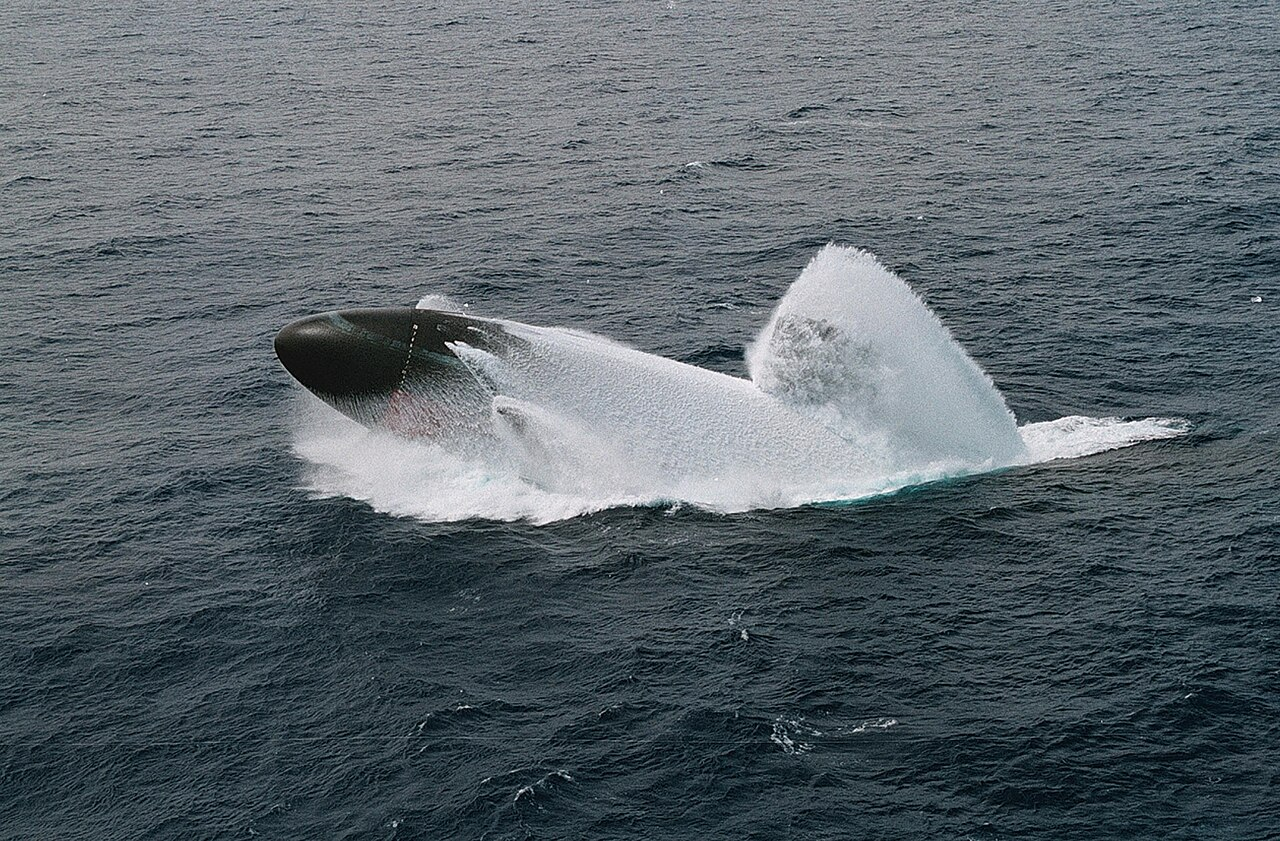
\includegraphics[width=0.60\linewidth]{images/book3/submarine-surfacing.jpg}

{\small Un submarino en un ejercicio de emersión de emergencia (Marina de los EE.\,UU.): vaciados sus lastres, pesa menos que el agua que desaloja y sube --- el \omterm{thm:b1:fluid-statics:archimedes}{teorema de Arquímedes} a \qty{7000}{t}.}
\end{omfigure}

\section{La presión en un fluido en reposo}

\begin{proposition}[Isotropía de la presión]\label{prop:b1:fluid-statics:isotropy}
\index{presión!en un fluido}
En un fluido en reposo, la fuerza que ejerce el fluido sobre una pequeña
superficie $\dd S$ situada en un punto $M$ es $\dd\vect F = P(M)\,\dd S\,\vect n$,
normal a la superficie y dirigida hacia ella, con una presión $P(M)$ que
depende del punto pero \emph{no} de la orientación de la superficie.
\end{proposition}

\begin{proof}[Demostración parcial]
Un fluido en reposo no transmite ninguna fuerza tangencial (si no,
fluiría): la fuerza es normal. Tómese un pequeño prisma triangular de
fluido en $M$ con caras de orientaciones distintas: está en equilibrio
bajo las fuerzas de presión sobre sus caras y su peso; el peso crece como
el volumen (el cubo del tamaño) y las fuerzas de presión como las áreas
(el cuadrado), de modo que en un prisma bastante pequeño solo cuentan las
fuerzas de presión, y su equilibrio en toda dirección exige el mismo $P$
sobre cada cara.
\end{proof}

\begin{theorem}[Relación fundamental de la estática de fluidos]\label{thm:b1:fluid-statics:fundamental}
\index{relación hidrostática}
En un fluido en reposo en la gravedad uniforme $\vect g = -g\vect e_z$ ($z$
hacia arriba), la presión solo depende de $z$ y
\[
\frac{\dd P}{\dd z} = -\rho g ,
\]
donde $\rho$ es la densidad del fluido a ese nivel. La presión crece hacia
abajo; las superficies de igual presión (las \emph{isobaras}) son
horizontales, y también lo es la superficie libre de un líquido.
\end{theorem}

\begin{proof}
Tómese una rodaja horizontal de fluido de área $S$ entre $z$ y $z + \dd z$:
la empuja hacia arriba $P(z)S$ por debajo, hacia abajo $P(z + \dd z)S$ por
encima, y hacia abajo su peso $\rho gS\,\dd z$. En reposo:
$P(z)S - P(z + \dd z)S - \rho gS\,\dd z = 0$. Una rodaja horizontal no
recibe fuerza horizontal de la gravedad, luego $P$ es uniforme en horizontal.
\end{proof}

\begin{omfigure}
\begin{tikzpicture}[font=\small, x=1cm, y=1cm]
  \fill[omDef!10] (-2.4,-1.8) rectangle (2.4,1.8);
  \draw[thick, fill=omDef!30] (-1.2,-0.25) rectangle (1.2,0.25);
  \draw[-Stealth, omThm, very thick] (0,-1.3) -- (0,-0.3) node[pos=0.0, below] {$P(z)\,S$};
  \draw[-Stealth, omThm, very thick] (0,1.3) -- (0,0.3) node[pos=0.0, above] {$P(z + \dd z)\,S$};
  \draw[-Stealth, omProp, very thick] (0.9,0) -- (0.9,-0.9) node[right] {$\rho gS\,\dd z$};
  \draw[Stealth-Stealth] (-1.5,-0.25) -- (-1.5,0.25) node[midway, left] {$\dd z$};
  \draw[-Stealth] (2.8,-1.5) -- (2.8,1.5) node[above] {$z$};
  \node[font=\footnotesize] at (0,-2.1) {$P(z) - P(z + \dd z) = \rho g\,\dd z$};
\end{tikzpicture}\qquad
\begin{tikzpicture}[font=\small, x=1cm, y=1cm]
  % communicating vessels
  \fill[omDef!25] (0,0) rectangle (0.8,2.4); \fill[omDef!25] (0,0) rectangle (4.2,0.6); \fill[omDef!25] (1.8,0) rectangle (2.4,2.4); \fill[omDef!25] (3.4,0) rectangle (4.2,2.4);
  \draw[thick] (0,3.2) -- (0,0) -- (4.2,0) -- (4.2,3.2); \draw[thick] (0.8,3.2) -- (0.8,0.6) -- (1.8,0.6) -- (1.8,3.2); \draw[thick] (2.4,3.2) -- (2.4,0.6) -- (3.4,0.6) -- (3.4,3.2);
  \draw[omDef, thick] (0,2.4) -- (0.8,2.4); \draw[omDef, thick] (1.8,2.4) -- (2.4,2.4); \draw[omDef, thick] (3.4,2.4) -- (4.2,2.4);
  \draw[dashed, omThm] (-0.3,2.4) -- (4.5,2.4); \node[omThm, right] at (4.5,2.4) {mismo nivel};
  \node[font=\footnotesize] at (2.1,-0.4) {mismo $P$ en una horizontal};
\end{tikzpicture}

{\small A la izquierda: equilibrio de una rodaja horizontal de fluido ---
la presión de abajo ha de superar a la de arriba en el peso de la rodaja
por unidad de área. A la derecha: vasos comunicantes --- una horizontal
encuentra la misma presión en todo el líquido conectado, de modo que las
superficies libres quedan a un mismo nivel sean cuales sean las formas.}
\end{omfigure}

\begin{corollary}[Fluido incompresible]\label{cor:b1:fluid-statics:incompressible}
\index{presión hidrostática}
En un líquido de densidad uniforme $\rho$, la presión a una profundidad $h$
por debajo de un punto donde vale $P_0$ es
\[
P = P_0 + \rho gh .
\]
Agua: \qty{1}{bar} más cada \qty{10}{m}. Dos puntos de un líquido
conectado situados al mismo nivel están a la misma presión; las
superficies libres de vasos comunicantes quedan a un mismo nivel; una
presión aplicada en cualquier punto de un líquido encerrado se transmite
íntegra a todos los demás (el principio de Pascal).
\end{corollary}

\begin{proof}
Intégrese $\dd P/\dd z = -\rho g$ con $\rho$ constante; lo demás es la
horizontalidad de las isobaras y la unicidad de $P$ en cada nivel.
\end{proof}

\begin{example}[Manómetros y prensas]\label{ex:b1:fluid-statics:manometer}
\index{manómetro}\index{prensa hidráulica}
Un tubo en U de mercurio ($\rho = \qty{13600}{kg/m^3}$) cuyas columnas
difieren en $h = \qty{760}{mm}$ mide una diferencia de presión
$\rho gh = \qty{1.013e5}{Pa}$ --- la atmósfera, que sostiene una columna de
agua de \qty{10.3}{m}. Una \omterm{ex:b1:fluid-statics:manometer}{prensa hidráulica}: una fuerza $F_1$ sobre un
pistón de área $S_1$ eleva la presión en $F_1/S_1$ en todo el líquido; sobre
el pistón grande $S_2$ da $F_2 = F_1S_2/S_1$ --- cincuenta veces más para
cincuenta veces el área, al precio de cincuenta veces menos recorrido (la
energía se conserva: $F_1d_1 = F_2d_2$).
\end{example}

\section{La atmósfera}

\begin{proposition}[Atmósfera isoterma]\label{prop:b1:fluid-statics:atmosphere}
\index{fórmula barométrica}\index{altura de escala}
Para un \omterm{def:b1:kinetic-theory:model}{gas perfecto} de masa molar $M$ a temperatura uniforme $T$ en una
gravedad uniforme,
\[
P(z) = P_0\,\eu^{-z/H}, \qquad H = \frac{RT}{Mg} ,
\]
la \emph{\omterm{prop:b1:fluid-statics:atmosphere}{altura de escala}}: unos \qty{8}{km} para el aire; la presión se
reduce a la mitad cada $H\ln2 \approx \qty{5.5}{km}$.
\end{proposition}

\begin{proof}
$\rho = PM/RT$ (ecuación de estado), luego $\dd P/\dd z = -(Mg/RT)P$: una
ecuación lineal de primer orden, $P = P_0\eu^{-Mgz/RT}$.
\end{proof}

\begin{example}[Aire enrarecido]\label{ex:b1:fluid-statics:altitude}
Con $T = \qty{260}{K}$ (una media de la atmósfera baja), $H =
\qty{7.6}{km}$: $P = 0.52P_0$ a \qty{5000}{m} y $0.31P_0$ en la cima del
Everest --- cerca de los valores medidos $0.54$ y $0.33$; la atmósfera real
se enfría con la altura, cosa que tiene en cuenta el volumen del Año 2. El
modelo dice además por qué el mar es distinto: el agua es ochocientas
veces más densa y casi incompresible, de modo que su presión crece
linealmente, un bar cada diez metros, sin \omterm{prop:b1:fluid-statics:atmosphere}{altura de escala}.
\end{example}

\begin{omfigure}
\begin{tikzpicture}
\begin{axis}[omaxis, axis x line=bottom, axis y line=left, width=8cm, height=5.4cm, xlabel={$z$ (\unit{km})}, ylabel={$P/P_0$},
    xlabel style={at={(axis description cs:0.5,-0.12)}, anchor=north},
    xmin=0, xmax=30, ymin=0, ymax=1.1, xtick={5.5,10,20,30}, xticklabels={$5.5$,$10$,$20$,$30$}, ytick={0.5,1}]
  \addplot[omDef, thick, domain=0:30, samples=100] {exp(-x/7.6)};
  \draw[dashed, omExo] (axis cs:0,0.5) -- (axis cs:5.3,0.5) -- (axis cs:5.3,0);
  \node[omDef, font=\footnotesize] at (axis cs:16,0.45) {$P_0\eu^{-z/H}$, $H = \qty{7.6}{km}$};
\end{axis}
\end{tikzpicture}

{\small La atmósfera isoterma: la presión (y la densidad) caen
exponencialmente con la altura y se reducen a la mitad cada \qty{5.5}{km}.
Nueve décimas partes del aire están por debajo de \qty{17}{km}.}
\end{omfigure}

\section{Fuerzas sobre las paredes}

\begin{proposition}[Fuerza sobre una pared vertical]\label{prop:b1:fluid-statics:wall}
\index{centro de presiones}
Un líquido de profundidad $h$ contra una pared vertical rectangular de
anchura $L$ (con la presión atmosférica actuando sobre ambas caras y
cancelándose) ejerce la fuerza horizontal
\[
F = \tfrac12\rho gh^2L ,
\]
equivalente a una fuerza única aplicada en el \emph{\omterm{prop:b1:fluid-statics:wall}{centro de presiones}}, a
la profundidad $2h/3$ --- la resultante actúa abajo, donde la presión es
mayor.
\end{proposition}

\begin{proof}
A la profundidad $x$ la presión manométrica vale $\rho gx$; sobre la banda
de altura $\dd x$ la fuerza es $\rho gxL\,\dd x$; intégrese de $0$ a $h$. Su
momento respecto de la línea de la superficie es
$\int_0^h\rho gx^2L\,\dd x = \tfrac13\rho gh^3L$; al dividir por $F$ se
obtiene el brazo $2h/3$.
\end{proof}

\begin{omfigure}
\begin{tikzpicture}[font=\small, x=1cm, y=1cm]
  \fill[omDef!20] (-3.6,0) rectangle (0,2.8);
  \draw[thick] (-3.8,2.8) -- (0,2.8); \draw[omDef, thick] (-3.6,2.8) -- (0,2.8);
  \draw[thick, fill=omExo!40] (0,0) -- (0,3.2) -- (1.0,3.2) -- (1.8,0) -- cycle;
  \draw[thick] (-3.8,0) -- (2.6,0);
  \foreach \y/\l in {2.5/0.15, 2.0/0.4, 1.5/0.65, 1.0/0.9, 0.5/1.15, 0.1/1.35} {\draw[-Stealth, omThm] (-\l,\y) -- (0,\y);}
  \draw[omThm, dashed] (0,2.8) -- (-1.4,0);
  \draw[-Stealth, omThm, very thick] (-2.6,0.93) -- (-0.05,0.93) node[pos=0.0, left] {$F = \tfrac12\rho gh^2L$};
  \draw[Stealth-Stealth] (2.2,2.8) -- (2.2,0.93) node[midway, right] {$\tfrac23 h$};
  \draw[Stealth-Stealth] (-3.2,2.8) -- (-3.2,0) node[midway, left] {$h$};
\end{tikzpicture}

{\small La presión sobre una presa crece linealmente con la profundidad
(flechas), de modo que la resultante actúa a dos tercios de la
profundidad: el muro ha de ser más grueso abajo. La fuerza depende de $h$
y de $L$, no de cuánta agua haya detrás.}
\end{omfigure}

\begin{example}[Una presa]\label{ex:b1:fluid-statics:dam}
$h = \qty{20}{m}$, $L = \qty{100}{m}$: $F = \tfrac12 \times 1000 \times 9.81 \times
400 \times 100 = \qty{2.0e8}{N}$ --- veinte mil toneladas, aplicadas
\qty{13}{m} por debajo de la superficie, lo mismo si detrás hay una charca
o un fiordo: la \emph{paradoja hidrostática}.
\end{example}

\section{El teorema de Arquímedes}

\begin{theorem}[Arquímedes]\label{thm:b1:fluid-statics:archimedes}
\index{teorema de Arquímedes}\index{empuje}\index{centro de empuje}
Un cuerpo sumergido en un fluido en reposo recibe de las fuerzas de
presión una resultante --- el \emph{empuje} --- igual y opuesta al peso del
fluido que desaloja,
\[
\vect\Pi = -\rho_{\text{fluido}}V_{\text{sumergido}}\,\vect g ,
\]
aplicada en el centro de masa del fluido desalojado (el \emph{\omterm{thm:b1:fluid-statics:archimedes}{centro de
empuje}}).
\end{theorem}

\begin{proof}
Las fuerzas de presión sobre la superficie del cuerpo solo dependen de la
forma de esa superficie y del fluido exterior. Sustitúyase el cuerpo, con
el pensamiento, por fluido en reposo que ocupe el mismo volumen: ese
fluido está en equilibrio bajo su peso y las mismas fuerzas de presión,
luego las fuerzas de presión equilibran su peso --- suman $-\rho V\vect g$,
aplicado en su centro de masa. Deshágase la sustitución imaginaria; las
fuerzas de presión no han cambiado.
\end{proof}

\begin{corollary}[Flotación]\label{cor:b1:fluid-statics:floating}
\index{flotación}
Un cuerpo de densidad $\rho_b$ flota en un fluido de densidad $\rho_f > \rho_b$
con la fracción $\rho_b/\rho_f$ de su volumen sumergida; si $\rho_b >
\rho_f$ se hunde, con un peso aparente $(\rho_b - \rho_f)Vg$.
\end{corollary}

\begin{proof}
El peso $\rho_bVg$ iguala al empuje $\rho_fV_{\text{sum}}g$.
\end{proof}

\begin{omfigure}
\begin{tikzpicture}[font=\small, x=1cm, y=1cm]
  \fill[omDef!15] (-3.6,-2.2) rectangle (3.6,0);
  \draw[omDef, thick] (-3.6,0) -- (3.6,0);
  % iceberg-like block: rectangle 2 x 1.6, 90% immersed
  \draw[thick, fill=white] (-1.0,-1.44) rectangle (1.0,0.16);
  \fill (0,-0.64) circle (1.5pt) node[right] {$G$};
  \fill[omDef] (0,-0.72) circle (1.5pt) node[left] {$C$};
  \draw[-Stealth, omThm, very thick] (0,-0.64) -- (0,-1.9) node[below] {$\rho_bVg$};
  \draw[-Stealth, omDef, very thick] (0,-0.72) -- (0,0.55) node[above] {$\rho_fV_{\text{sum}}g$};
  \node[font=\footnotesize] at (2.4,-1.2) {$\dfrac{V_{\text{sum}}}{V} = \dfrac{\rho_b}{\rho_f}$};
\end{tikzpicture}

{\small Un cuerpo que flota: su peso, aplicado en su centro de masa $G$,
equilibra al empuje, aplicado en el \omterm{thm:b1:fluid-statics:archimedes}{centro de empuje} $C$ (el centro del
volumen sumergido). Hielo ($\rho = \qty{917}{kg/m^3}$) en agua de mar
($\qty{1025}{kg/m^3}$): un $89\%$ bajo la superficie.}
\end{omfigure}

\begin{example}[Tres empujes]\label{ex:b1:fluid-statics:buoy}
Un densímetro es un tubo lastrado que se hunde hasta desalojar su propio
peso: cuanto más denso es el líquido, menos se hunde --- un medidor de
densidad que se lee en su vástago. Un globo de \qty{2800}{m^3} de aire
caliente a \qty{373}{K} desaloja \qty{3.4}{t} de aire frío y pesa
\qty{2.6}{t} de aire caliente: \qty{0.7}{t} de fuerza ascensional
(\cref{pb:b1:kinetic-theory:1}). Un buque de \qty{100000}{t} desaloja
\qty{97600}{m^3} de agua de mar; en agua dulce ($\qty{1000}{kg/m^3}$) ha de
desalojar un $2.5\%$ más y se hunde más --- las marcas de francobordo de su
casco.
\end{example}

\begin{remark}[Estabilidad]\label{rem:b1:fluid-statics:stability}
\index{metacentro}
Un cuerpo que flota inclinado un ángulo pequeño se endereza si el empuje,
aplicado ahora en el centro desplazado del nuevo volumen sumergido, produce
un momento restaurador --- lo que ocurre cuando el \emph{metacentro} (el
punto donde la recta de acción del empuje corta al eje del cuerpo) queda
por encima de $G$. El lastre en el fondo de la bodega baja $G$ y estabiliza
el buque; una embarcación con demasiado peso arriba vuelca.
\end{remark}

\section{Ejercicios}

\begin{exercise}[$\star$]\label{exo:b1:fluid-statics:1}
Presión absoluta a \qty{10}{m}, \qty{100}{m} y \qty{1}{km} bajo el mar
($\rho = \qty{1025}{kg/m^3}$); fuerza sobre un portillo de \qty{1.0}{m^2} a
\qty{300}{m}.
\end{exercise}

\begin{exercise}[$\star$]\label{exo:b1:fluid-statics:2}
Altura de una columna de mercurio que equilibra \qty{1.013e5}{Pa}; y de una
de agua. ¿Por qué no puede una bomba aspirante elevar el agua más de unos
\qty{10}{m}?
\end{exercise}

\begin{exercise}[$\star$]\label{exo:b1:fluid-statics:3}
Un gato hidráulico: \qty{100}{N} sobre un pistón de \qty{2.0}{cm^2}, carga
sobre un pistón de \qty{200}{cm^2}; recorrido de cada uno si el pistón
pequeño avanza \qty{20}{cm}.
\end{exercise}

\begin{exercise}[$\star$]\label{exo:b1:fluid-statics:4}
Un tubo en U contiene agua; se vierte aceite ($\rho = \qty{850}{kg/m^3}$) en
una de las ramas y forma una columna de \qty{12}{cm}. Diferencia de altura
entre las dos superficies libres.
\end{exercise}

\begin{exercise}[$\star\star$]\label{exo:b1:fluid-statics:5}
\omterm{prop:b1:fluid-statics:atmosphere}{Altura de escala} de la atmósfera a \qty{273}{K}; presión a \qty{5000}{m} y a
\qty{8848}{m}; altura a la que $P = P_0/2$. Compárese con los valores
citados en \cref{ch:b1:kinetic-theory}.
\end{exercise}

\begin{exercise}[$\star\star$]\label{exo:b1:fluid-statics:6}
Una presa rectangular de \qty{100}{m} de anchura retiene \qty{20}{m} de
agua. Fuerza total, profundidad del \omterm{prop:b1:fluid-statics:wall}{centro de presiones} y momento del agua
respecto de la base de la presa. ¿Por qué se curva una presa hacia el agua?
\end{exercise}

\begin{exercise}[$\star\star$]\label{exo:b1:fluid-statics:7}
Fracción de un iceberg que queda bajo la superficie (hielo \qty{917}{kg/m^3},
agua de mar \qty{1025}{kg/m^3}); y de un tronco de densidad
\qty{600}{kg/m^3} en agua dulce; ¿a cuántas personas de \qty{75}{kg} puede
llevar una balsa de \qty{2.0}{m^3} de esa madera antes de que la cubierta
quede al ras del agua?
\end{exercise}

\begin{exercise}[$\star\star$]\label{exo:b1:fluid-statics:8}
Un densímetro de \qty{20}{g} con un vástago de sección \qty{0.50}{cm^2}
flota en agua con \qty{4.0}{cm} de vástago fuera. ¿Cuánto vástago emerge en
una salmuera de densidad \qty{1100}{kg/m^3}? ¿Sensibilidad (cm por unidad
de densidad relativa)?
\end{exercise}

\begin{exercise}[$\star\star$]\label{exo:b1:fluid-statics:9}
Un submarino de \qty{3000}{m^3} tiene una masa de \qty{2800}{t} con los
lastres vacíos. Fracción emergida en la superficie (agua de mar); masa de
agua que ha de tomar para quedar en flotabilidad neutra; ¿y si entra
después en un estuario de agua dulce?
\end{exercise}

\begin{exercise}[$\star\star\star$]\label{exo:b1:fluid-statics:10}
Un globo de niño contiene \qty{10}{L} de helio ($M = \qty{4}{g/mol}$) a
\qty{1}{bar} y \qty{293}{K}; la goma pesa \qty{3.0}{g}. Fuerza ascensional
neta; masa de cordel que puede llevar.
\end{exercise}

\begin{exercise}[$\star\star\star$]\label{exo:b1:fluid-statics:11}
Demuéstrese que el \omterm{prop:b1:fluid-statics:wall}{centro de presiones} sobre una pared vertical rectangular
está a $2h/3$ calculando el momento de las fuerzas de presión respecto de
la línea de la superficie. ¿Dónde está en una pared sumergida solo en
parte, digamos desde la profundidad $h_1$ hasta $h_2$?
\end{exercise}

\begin{exercise}[$\star\star\star$]\label{exo:b1:fluid-statics:12}
Un densímetro cilíndrico (masa $m$, sección $S$) que flota en un líquido de
densidad $\rho$ se hunde una longitud $x$ y se suelta. Muéstrese que
oscila armónicamente y dese el periodo; calcúlese para $m =
\qty{20}{g}$, $S = \qty{0.50}{cm^2}$, en agua. (\cref{ex:b1:oscillators-resonance:bob}
de nuevo.)
\end{exercise}

\begin{omfigure}
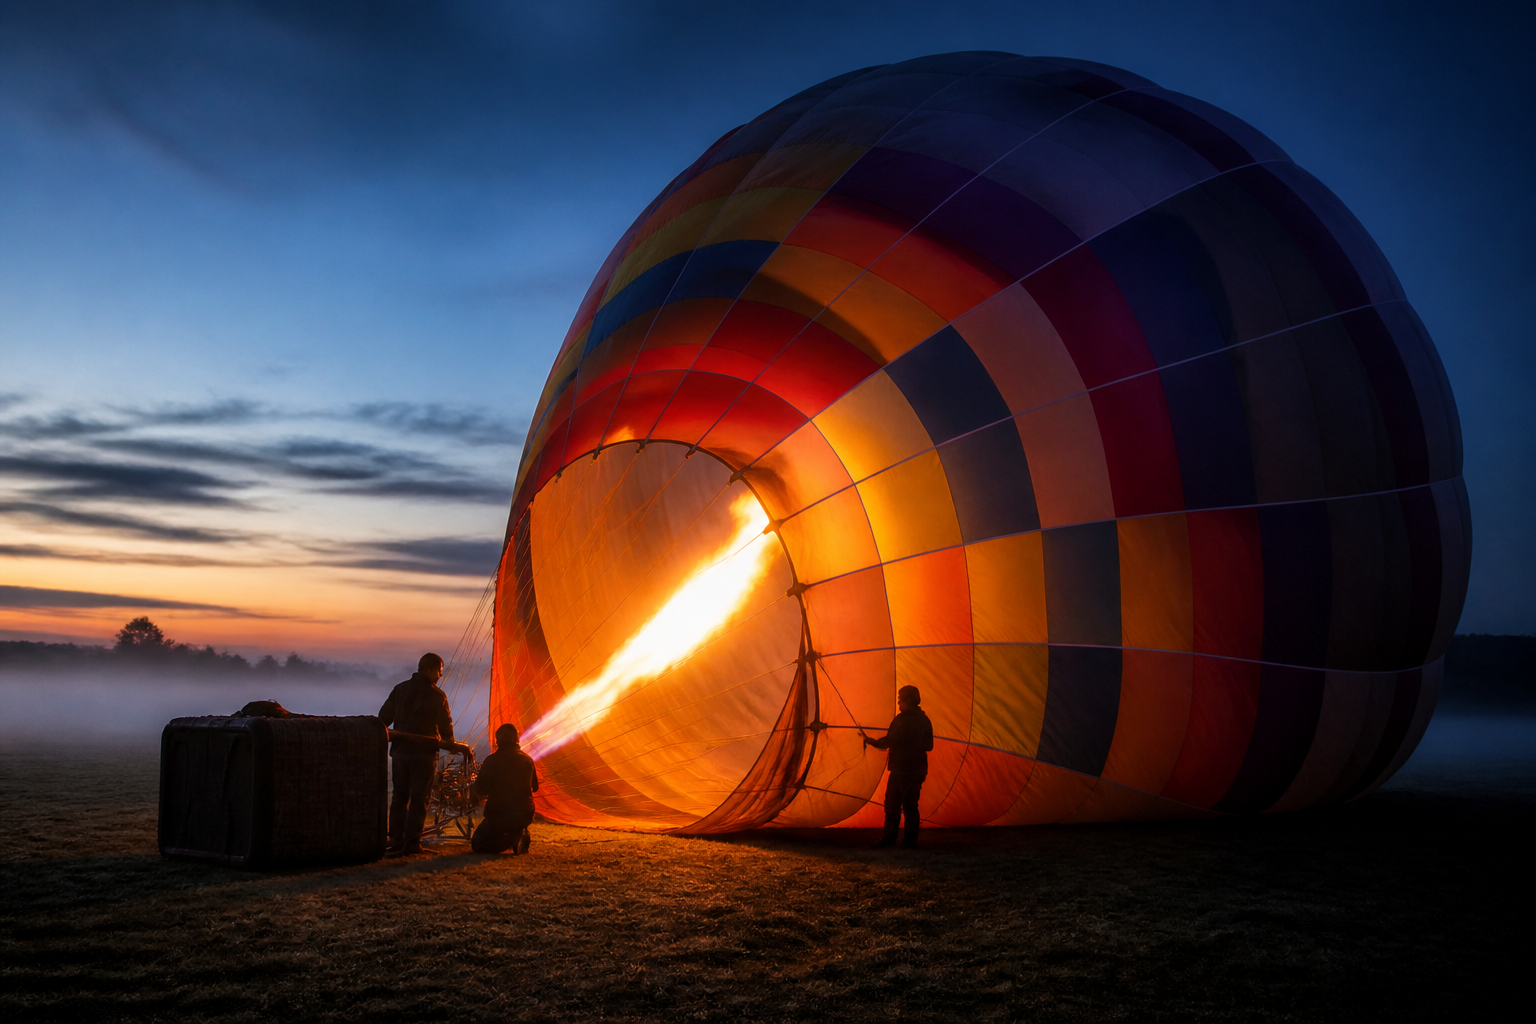
\includegraphics[width=0.58\linewidth]{images/book3/ai/b3-20-hot-air-balloon-burner.png}

{\small Inflado de un globo aerostático: el aire caliente es menos denso que el aire frío que lo rodea, y el empuje de Arquímedes sobre la envoltura supera a su peso.}
\end{omfigure}

\section{Problema: el submarino}

\begin{problem}[{Problema de fin de semana --- un casco de acero a
trescientos metros de profundidad: la presión sobre sus planchas, el agua
que ha de tragar para hundirse y escupir para subir, la buceadora que sale
de él y el petrolero que pasa por encima}]
\label{pb:b1:fluid-statics:1}
Agua de mar: $\rho = \qty{1025}{kg/m^3}$; agua dulce \qty{1000}{kg/m^3};
$P_0 = \qty{1.013e5}{Pa}$; $g = \qty{9.81}{m/s^2}$. El casco del submarino
encierra $V = \qty{3000}{m^3}$; con los lastres vacíos su masa es
$m_0 = \qty{2800}{t}$.

\medskip
\noindent\textbf{Parte I --- La presión sobre el casco.}
\begin{enumerate}
  \item Presión absoluta a \qty{300}{m}, en \omterm{def:b1:kinetic-theory:pressure}{pascales} y en bares.
  \item Fuerza sobre una escotilla circular de \qty{0.80}{m} de diámetro a
        esa profundidad; compárese con el peso de un camión.
  \item Fuerza sobre un metro cuadrado de casco en la quilla si el casco
        mide \qty{10}{m} de alto y su parte superior está a \qty{300}{m}:
        ¿cuánto difiere de la de arriba?
  \item El agua es ligeramente compresible ($\chi_T = \qty{4.6e-10}{Pa^{-1}}$):
        ¿en qué fracción es más densa el agua de mar a \qty{300}{m} que en
        la superficie? ¿Importa para la presión calculada antes?
  \item La tripulación respira aire a \qty{1}{atm}: ¿por qué ha de ser el
        casco un cilindro grueso, y por qué resiste mejor un cilindro que
        una caja plana?
  \item Una envolvente cilíndrica delgada de radio $R$ y espesor de pared $e$
        sometida a una sobrepresión exterior $\Delta P$ soporta en su pared
        una tensión de compresión $\Delta P\,R/e$. Para $R = \qty{5.0}{m}$ y
        $e = \qty{3.0}{cm}$ a \qty{300}{m}, calcúlese y compárese con el
        límite elástico del acero, de unos \qty{600}{MPa}.
\end{enumerate}

\medskip
\noindent\textbf{Parte II --- Hundirse y flotar.}
\begin{enumerate}[resume]
  \item En la superficie con los lastres vacíos, ¿qué volumen del casco
        emerge?
  \item ¿Qué masa de agua de mar han de tomar los lastres para que el
        submarino quede suspendido (flotabilidad neutra)?
  \item Ya en flotabilidad neutra a \qty{300}{m}, la presión comprime el
        casco un $0.1\%$. Calcúlese la fuerza neta resultante y dígase si el
        equilibrio es estable respecto de la profundidad.
  \item El buque navega en flotabilidad neutra del mar a un estuario de
        agua dulce. ¿Fuerza neta? ¿Hacia dónde va y qué ha de hacer la
        tripulación?
  \item Se lanza un torpedo de \qty{20}{t}. ¿Qué ha de hacer de inmediato el
        sistema de lastres, y en qué medida?
  \item ¿Por qué usa un submarino aire comprimido para vaciar sus lastres, y
        por qué es la presión del aire el límite de la profundidad a la que
        puede vaciarlos?
  \item Estímese el volumen de aire a \qty{1}{atm} necesario para vaciar
        \qty{275}{m^3} de lastres a \qty{300}{m} (ley de Boyle, $PV$
        constante).
\end{enumerate}

\medskip
\noindent\textbf{Parte III --- La buceadora.}
Una buceadora deja la superficie con \qty{6.0}{L} de aire en los pulmones.
\begin{enumerate}[resume]
  \item Presión absoluta a \qty{10}{m} y a \qty{30}{m}.
  \item Si desciende conteniendo la respiración, ¿cuál es el volumen de sus
        pulmones a \qty{30}{m}?
  \item Una buceadora con botella respira aire a la presión ambiente a
        \qty{30}{m} y asciende conteniendo la respiración: volumen que
        necesitarían sus pulmones en la superficie, y la lección.
  \item Un tubo respirador de \qty{1.0}{m}: diferencia de presión entre el
        agua sobre el pecho de la buceadora y el aire de sus pulmones;
        fuerza sobre un pecho de \qty{0.05}{m^2}; ¿puede inspirar?
  \item La botella contiene \qty{12}{L} a \qty{200}{bar}: ¿cuántos litros de
        aire a \qty{30}{m} son, y para cuánto tiempo a \qty{20}{L} por
        minuto?
\end{enumerate}

\medskip
\noindent\textbf{Parte IV --- El petrolero que pasa por encima.}
\begin{enumerate}[resume]
  \item Un petrolero de \qty{100000}{t} flota en agua de mar: volumen de
        agua desalojada.
  \item Su área de flotación es de \qty{8000}{m^2}: ¿cuánto sube o baja al
        entrar en agua dulce?
  \item Carga \qty{10000}{t} de petróleo: variación del calado.
  \item El petrolero vacío tiene el centro de masa alto; por eso lleva agua
        de mar como lastre cuando va sin carga. ¿Por qué, en términos del
        metacentro?
  \item El casco del petrolero en su quilla (calado de \qty{20}{m}): presión
        y fuerza por metro cuadrado, comparadas con las del submarino a
        \qty{300}{m}.
  \item El petrolero pasa justo por encima del submarino. ¿Nota el submarino
        sus \qty{100000}{t}? Explíquese con el campo de presiones.
  \item Resúmase: la única relación que ha fijado todos los números de este
        problema, y el teorema que se dedujo de ella.
\end{enumerate}
\end{problem}
